\chapter{Resultados y Discusión}

\section{Convergencia}

El proceso de optimización se extendió a lo largo de 590 épocas, observándose un régimen de estabilización asintótica en el tramo final. La evolución de la función de coste compuesta (MSTFT + EDC) muestra un descenso sostenido y coherente entre entrenamiento y validación. Tal como se aprecia en la Figura~\ref{fig:loss_curves}, la curva de validación sigue de manera estrecha la trayectoria de entrenamiento y se mantiene en valores equivalentes o inferiores, alcanzando niveles en el entorno de 9.42. Este patrón descarta de forma consistente la presencia de sobreajuste (\textit{overfitting}) y respalda la capacidad de generalización del modelo ante recintos no observados. Las oscilaciones de alta frecuencia, visibles tras superponer una tendencia suavizada por media móvil, se interpretan como un efecto inherente a la sensibilidad paramétrica de arquitecturas de Procesamiento Digital de Señal Diferenciable (DDSP).

\begin{figure}[htbp]
\centering
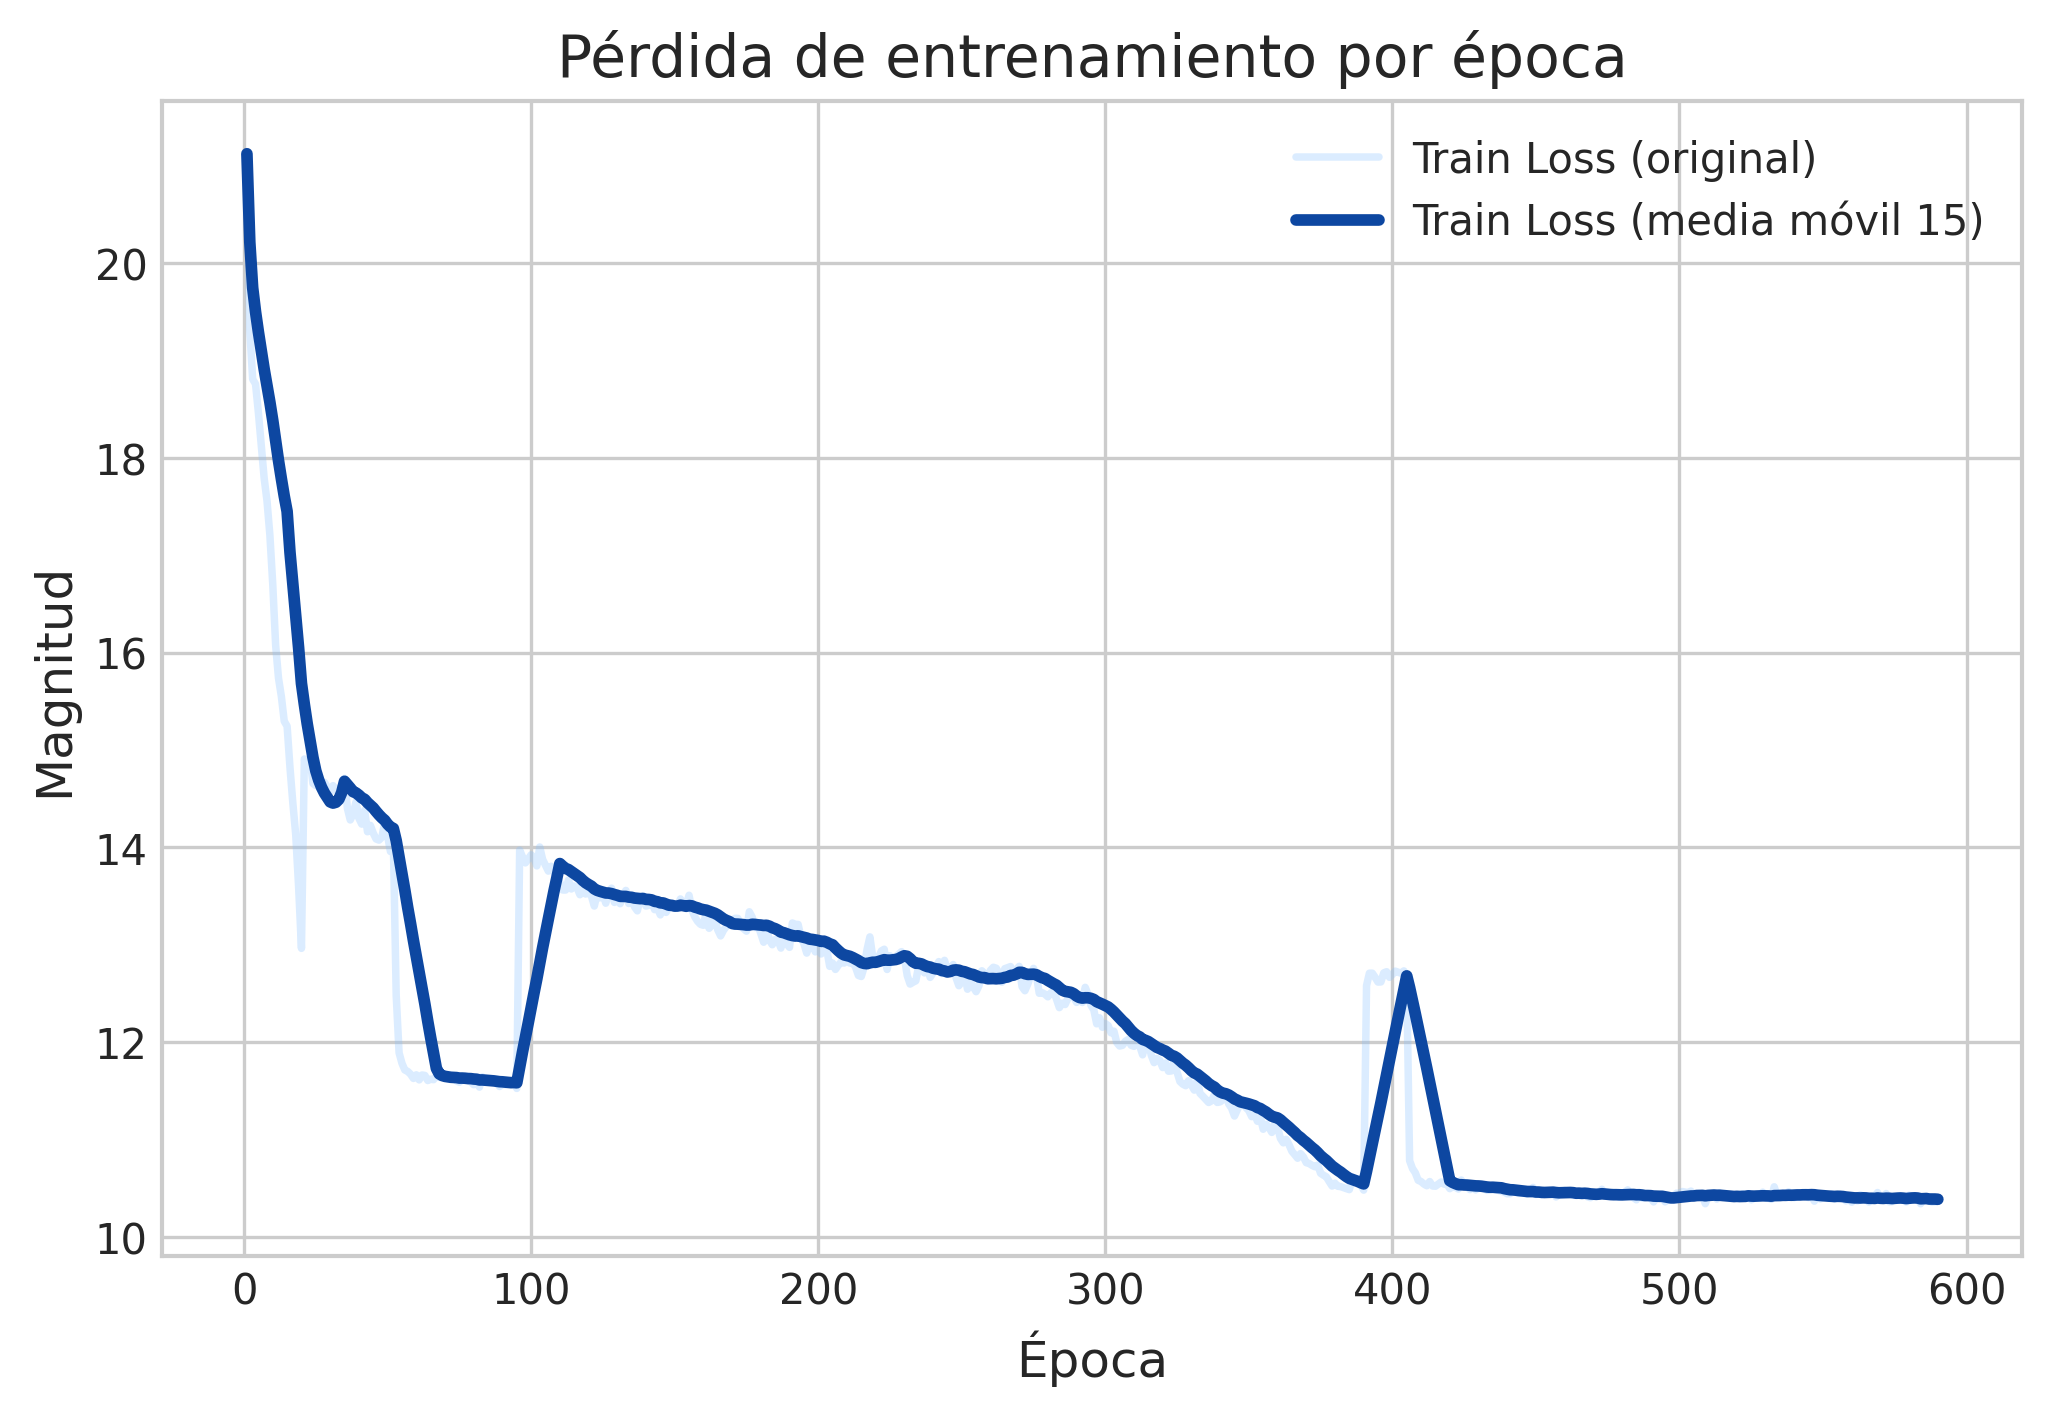
\includegraphics[width=0.48\textwidth]{../Figures/train_loss.png}
\hfill
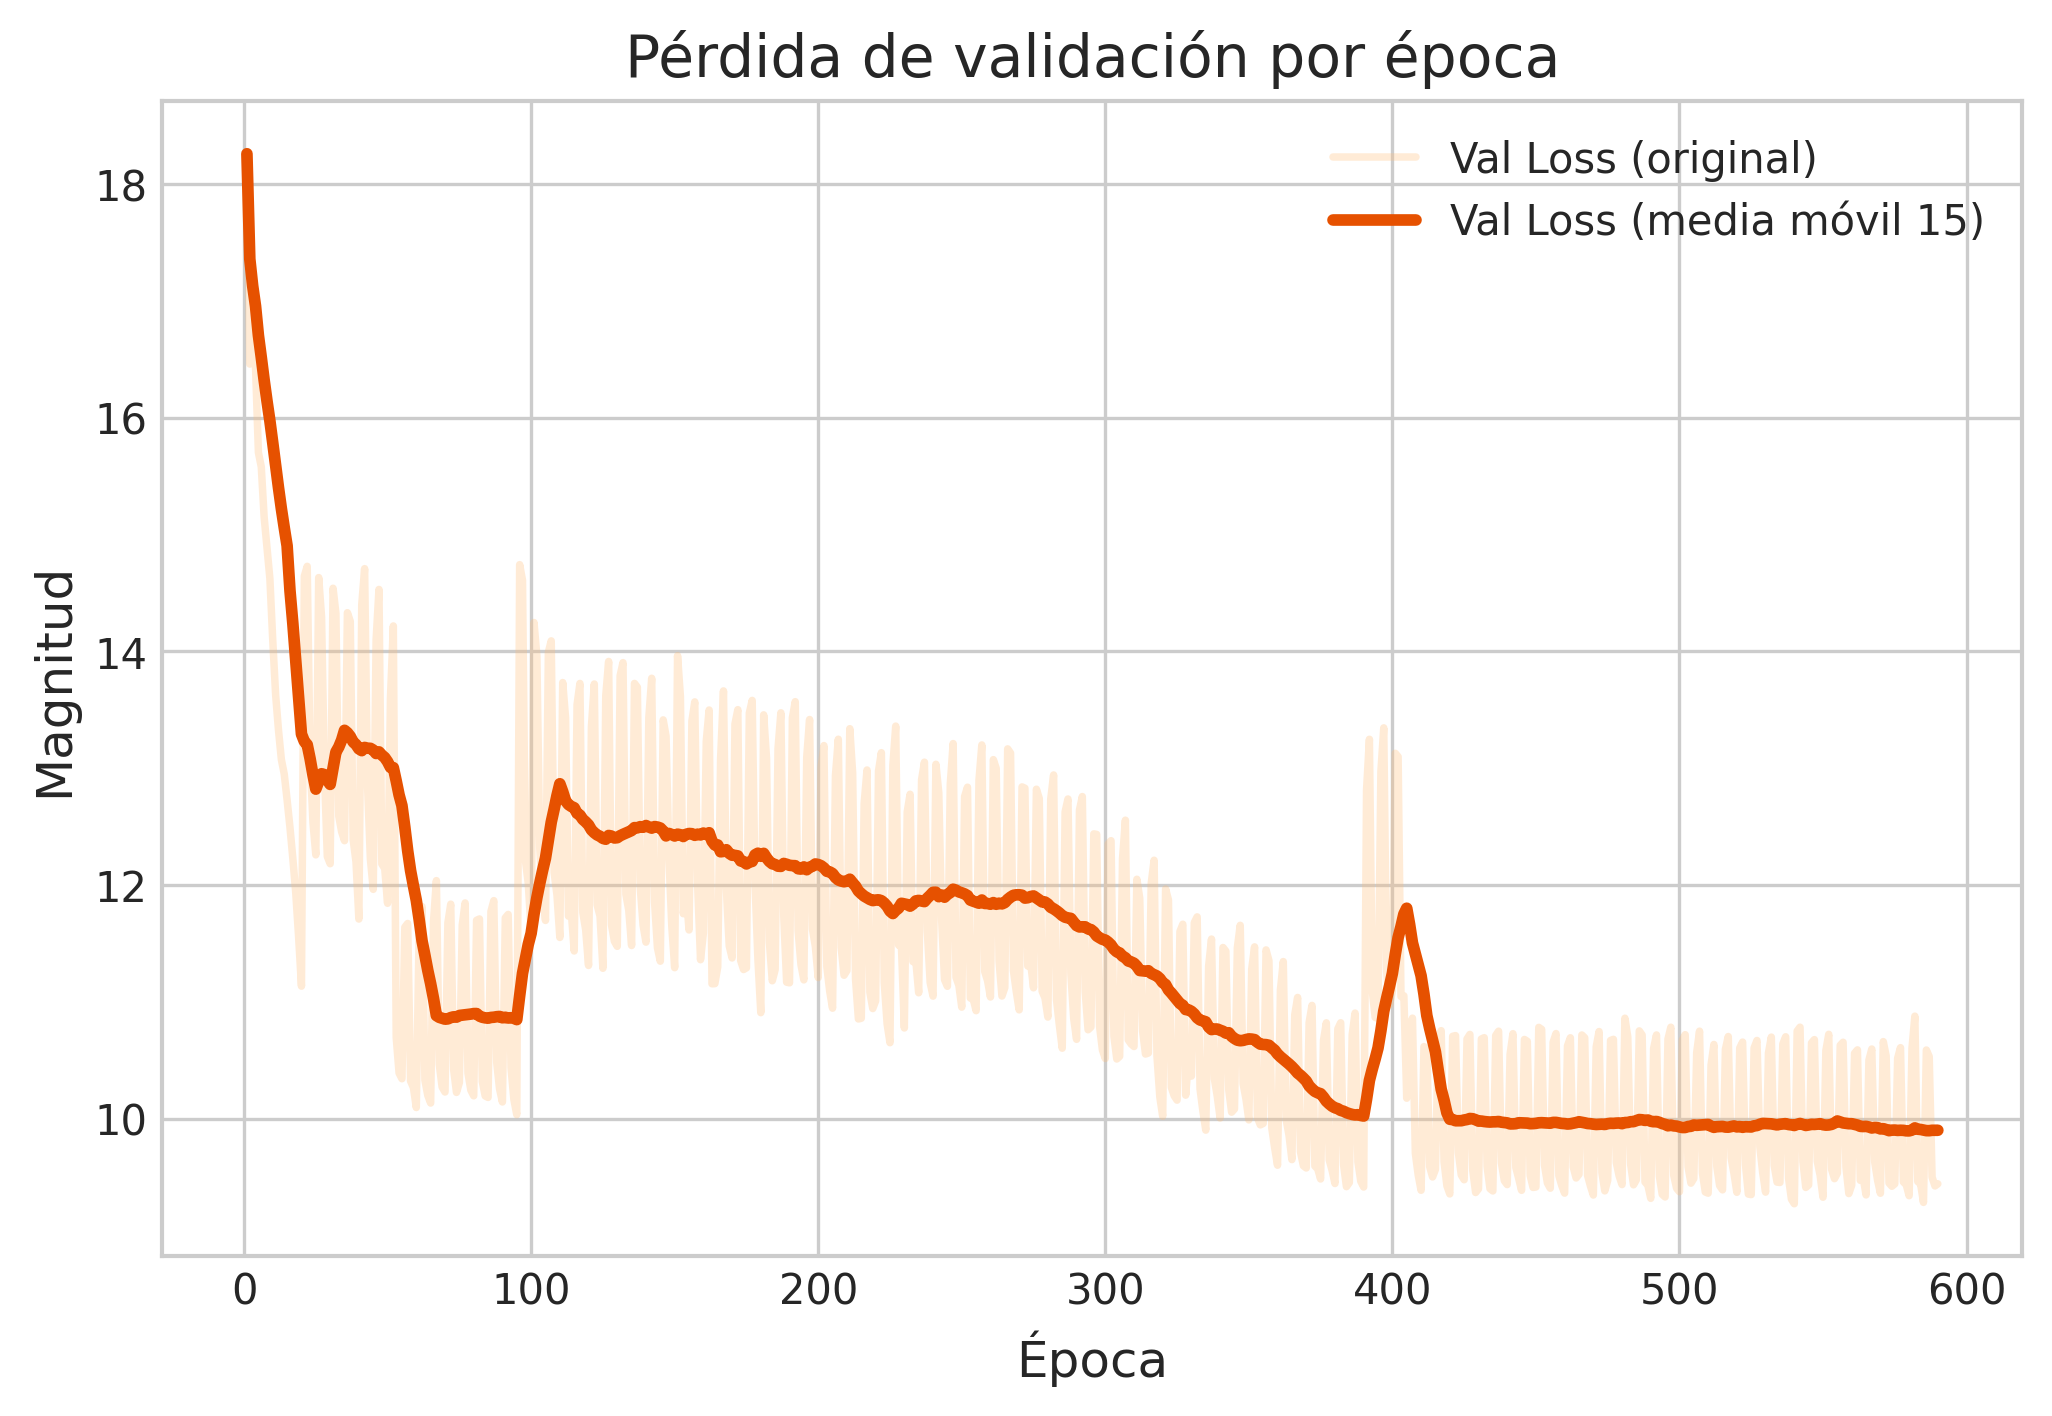
\includegraphics[width=0.48\textwidth]{../Figures/val_loss.png}
\caption{Evolución de la pérdida compuesta de entrenamiento y validación. Se superpone la tendencia suavizada mediante media móvil.}
\label{fig:loss_curves}
\end{figure}

La métrica física principal, definida como error absoluto medio sobre la Curva de Decaimiento de Energía (EDC-L1), presenta convergencia robusta durante el entrenamiento. En particular, la trayectoria perfora el umbral de 0.10 y se consolida en torno a 0.08 en las épocas finales, tal como se observa en la Figura~\ref{fig:edc_curves}. Este comportamiento confirma que la red no solo reduce error espectral, sino que también preserva la dinámica energética del decaimiento reverberante con precisión físicamente consistente.

\begin{figure}[htbp]
\centering
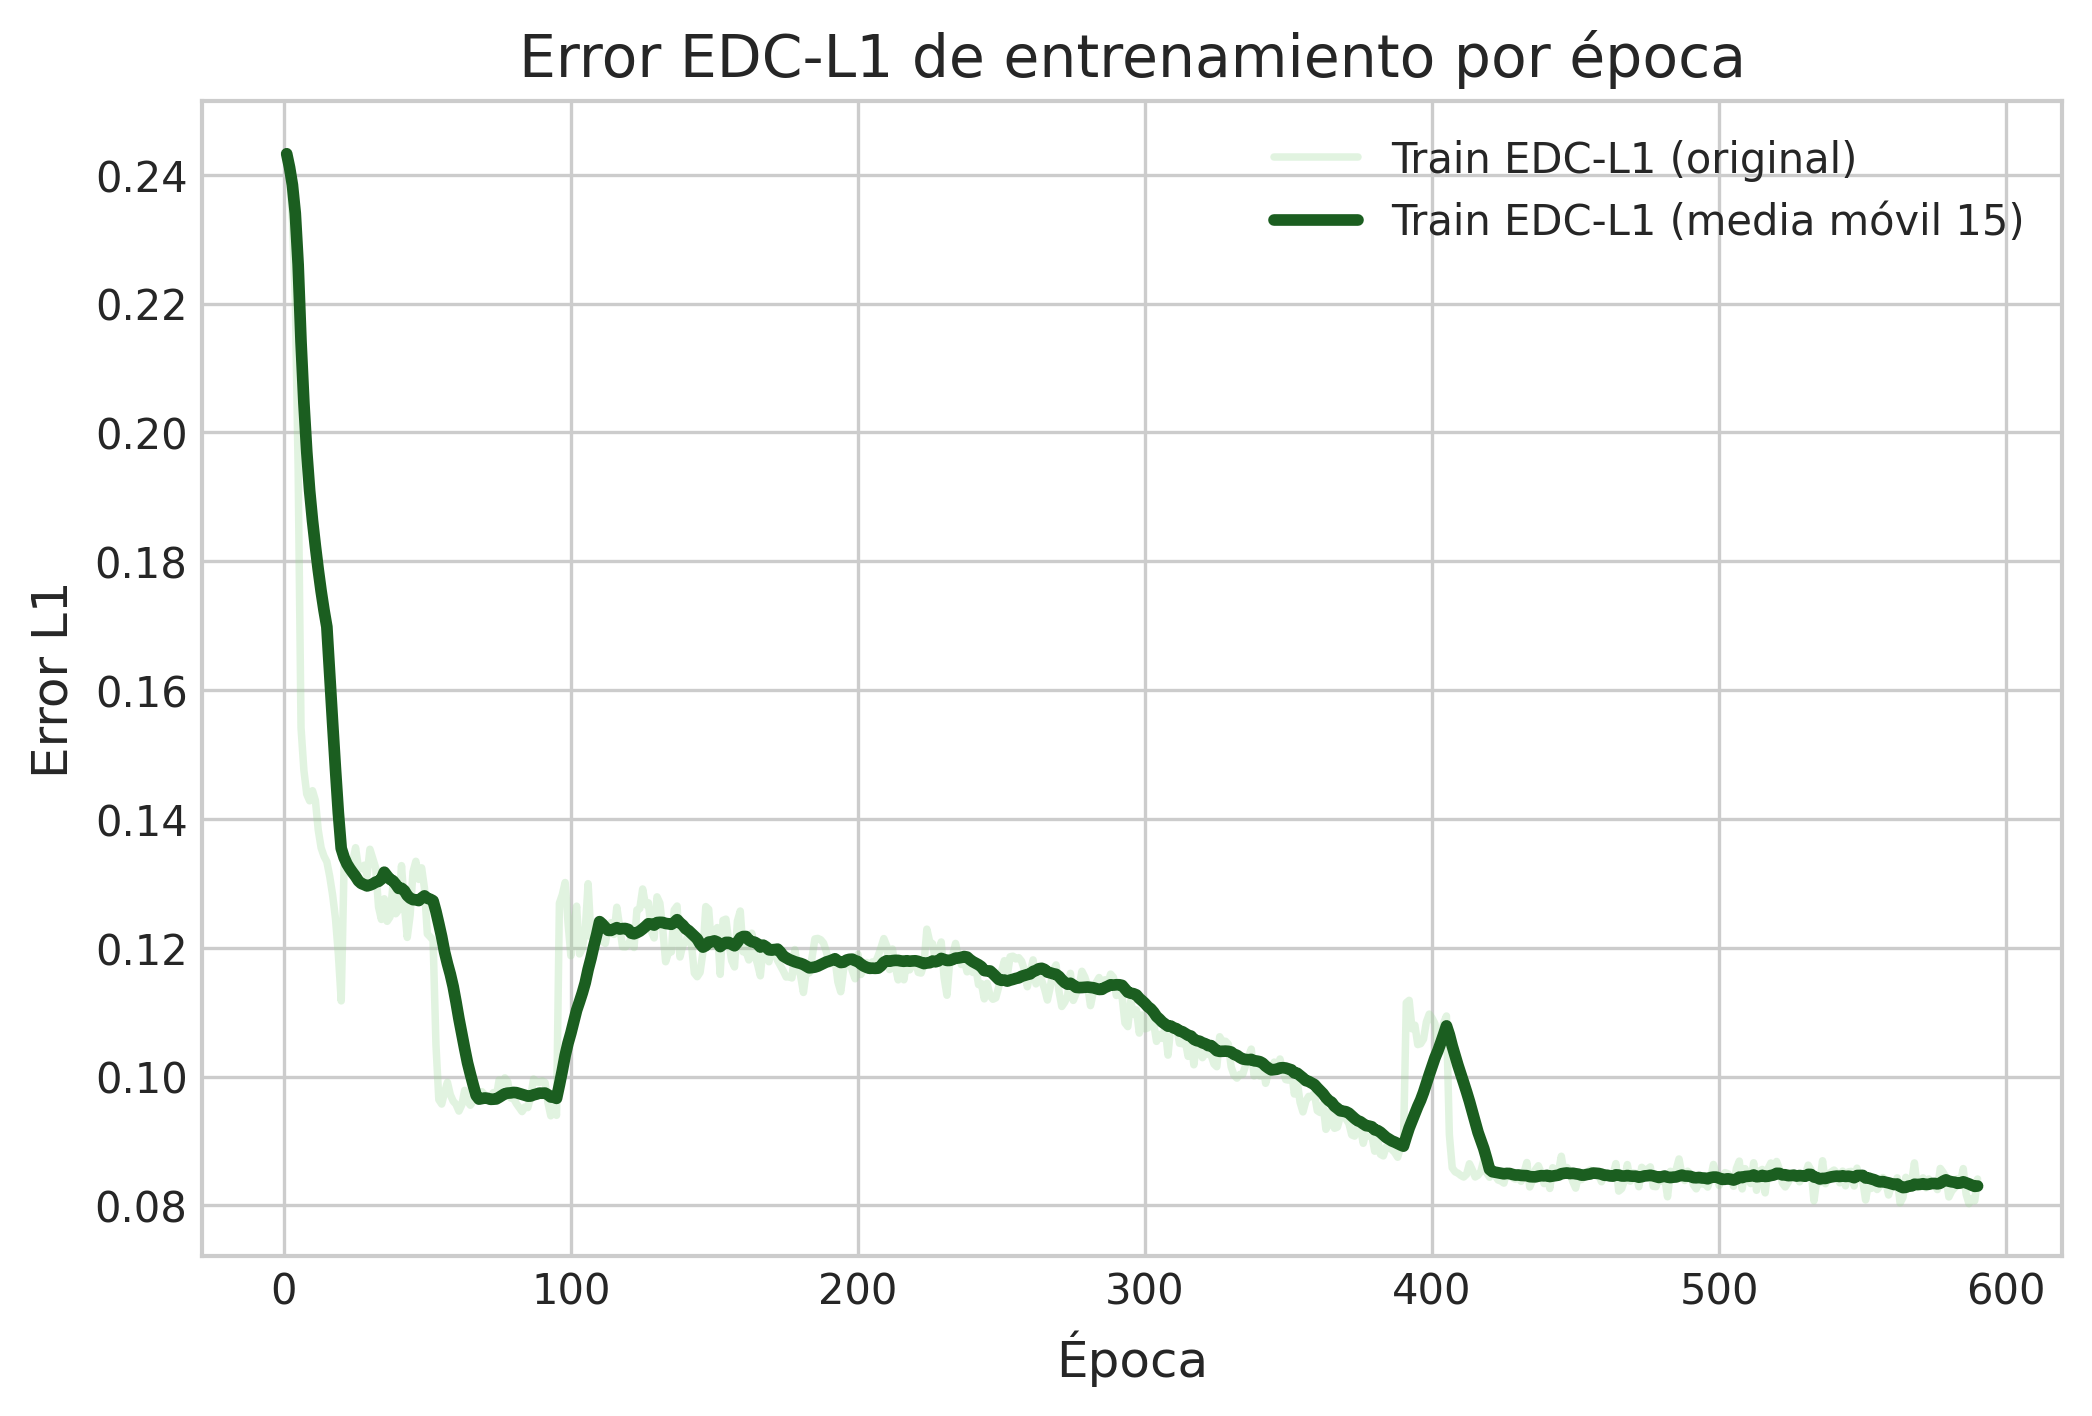
\includegraphics[width=0.48\textwidth]{../Figures/train_edc.png}
\hfill
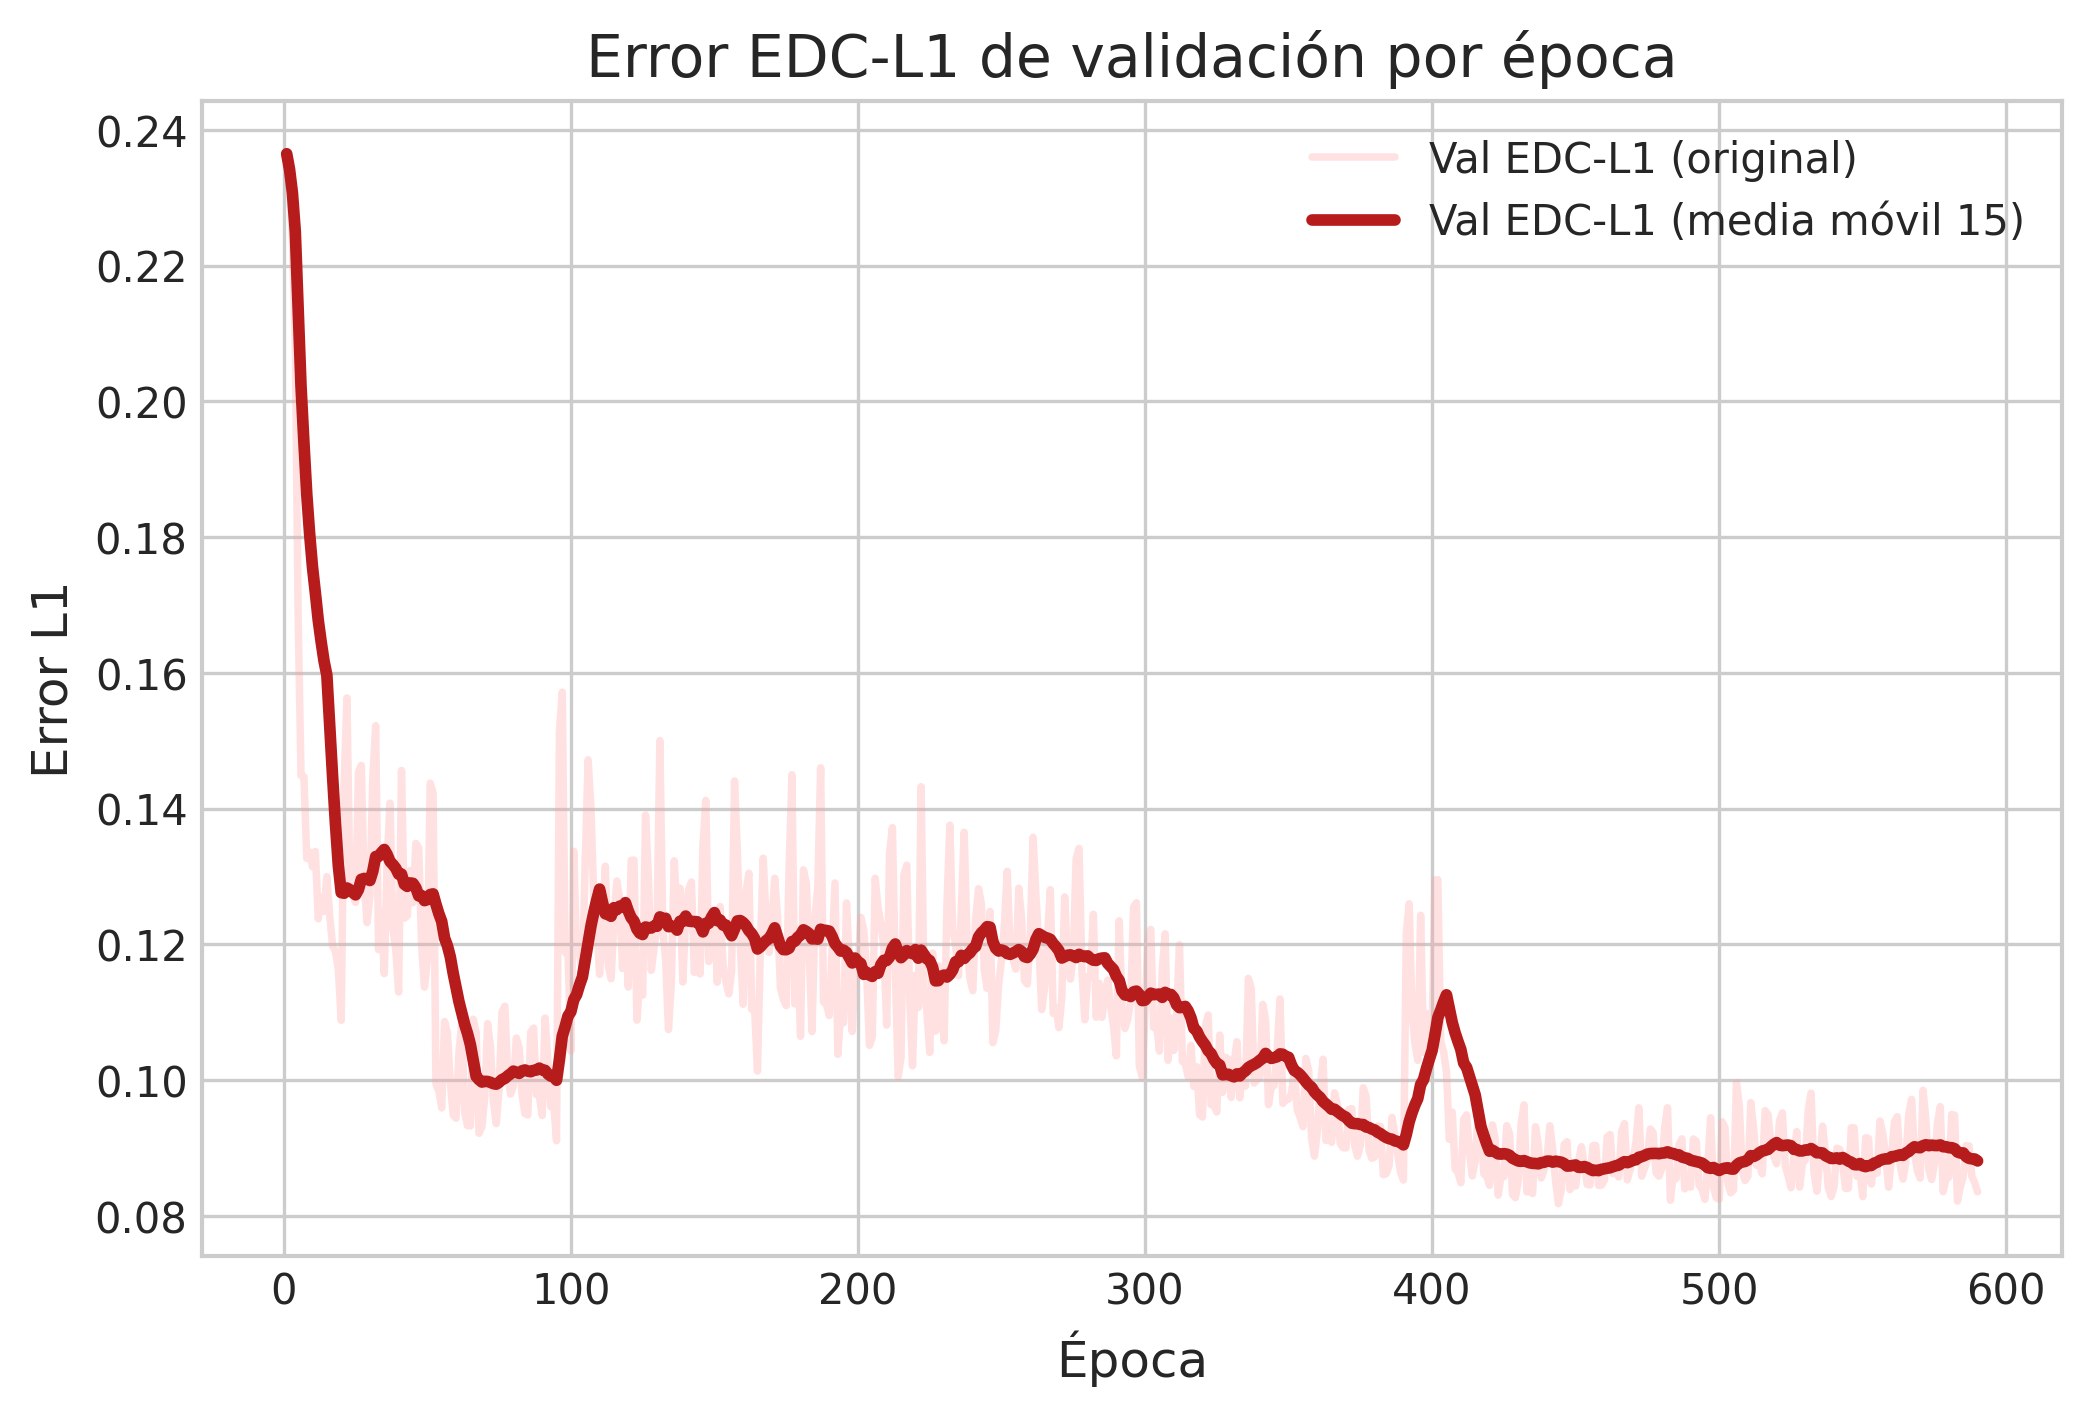
\includegraphics[width=0.48\textwidth]{../Figures/val_edc.png}
\caption{Convergencia del error absoluto medio de la Curva de Decaimiento de Energía (EDC-L1).}
\label{fig:edc_curves}
\end{figure}

Desde la perspectiva de estabilidad numérica, la predicción de tasas de decaimiento exponencial $b_k$ en el decodificador induce una superficie de pérdida fuertemente no convexa. La monitorización de la norma del gradiente, representada en la Figura~\ref{fig:gnorm}, evidencia picos transitorios severos que superan magnitudes del orden de $10^{4}$. Esta observación empírica justifica con rigor la necesidad técnica de emplear recorte de gradientes (\textit{gradient clipping}) dentro de Ranger21, mecanismo que resultó determinante para absorber inestabilidades locales y prevenir colapso numérico en los tensores durante fases críticas del aprendizaje.

\begin{figure}[htbp]
\centering
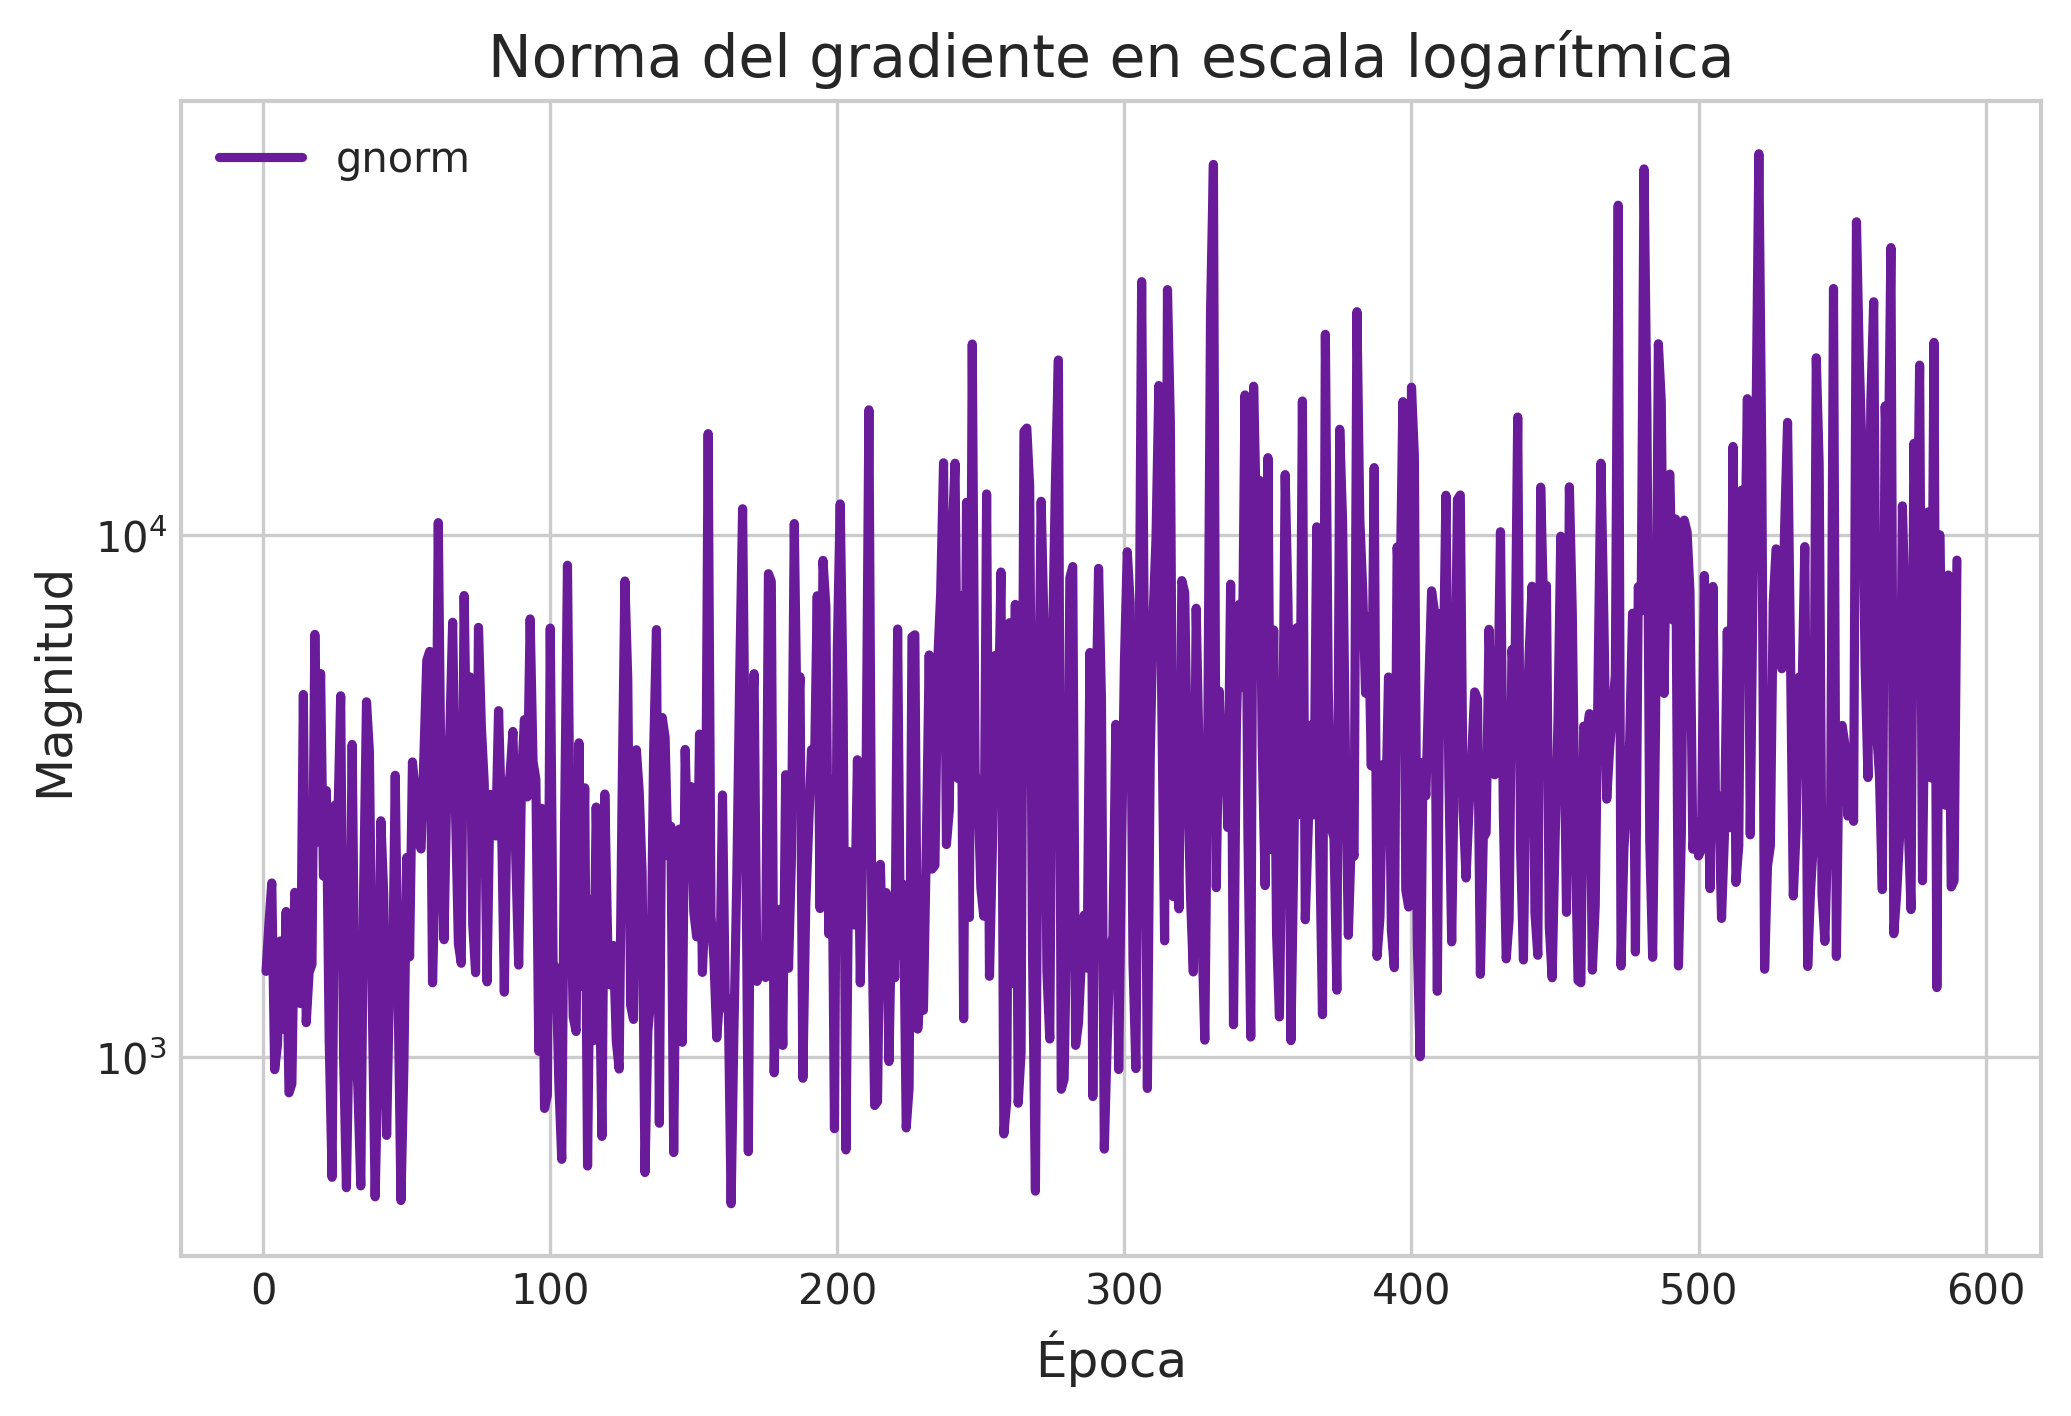
\includegraphics[width=0.75\textwidth]{../Figures/gnorm_log.png}
\caption{Evolución de la norma del gradiente en escala logarítmica durante el entrenamiento.}
\label{fig:gnorm}
\end{figure}

\section{Evaluación}

La validación cuantitativa del sistema se ha llevado a cabo sobre el subconjunto de test, compuesto por 40.000 muestras correspondientes a recintos no observados durante la fase de optimización. Para la inferencia se ha empleado el punto de control óptimo (\textit{checkpoint}) extraído en la época 540. El rendimiento se cuantifica mediante una doble perspectiva: por un lado, la fidelidad espectral global de la respuesta sintetizada y, por otro, la consistencia de descriptores acústicos físicos derivados de la Curva de Decaimiento de Energía (EDF).

\begin{lstlisting}[style=pythoncell,caption={Ejecución de la evaluación cuantitativa sobre el conjunto de test/validación.},label={lst:eval_run}]
CHECKPOINT_FINAL="/content/drive/MyDrive/TFG_Checkpoints/decor_v5_FINAL_ORO.pth"
DATA_LOCAL="/content/BIRD_Local"
python scripts/eval.py \
	--checkpoint "$CHECKPOINT_FINAL" \
	--data-root "$DATA_LOCAL"
\end{lstlisting}

\begin{table}[htbp]
\centering
\small
\setlength{\tabcolsep}{6pt}
\begin{tabular}{p{0.72\textwidth}r}
\toprule
\textbf{Métrica} & \textbf{Valor Medio ($\mu$)} \\
\midrule
Error Espectral Multiresolución (MSTFT) & 8.6108 \\
Error Absoluto Medio de la EDF (EDF MAE) [dB] & 5.39 \\
Raíz del Error Cuadrático Medio de la EDF (EDF RMSE) [dB] & 7.26 \\
Error Porcentual Absoluto Medio del $T_{60}$ ($T_{60}$ MAPE) [\%] & 8.1 \\
Error Cuadrático Medio de la Relación Directo-Reverberante (DRR MSE) [dB] & 7.24 \\
\bottomrule
\end{tabular}
\caption{Métricas de evaluación objetiva sobre el conjunto de test. Se reportan los valores medios obtenidos tras procesar las 40.000 muestras de evaluación.}
\label{tab:eval_objetiva}
\end{table}

Tal como se resume en la Tabla~\ref{tab:eval_objetiva}, el error MSTFT de 8.6108 cuantifica la fidelidad global de la distribución de energía espectrogramática y refleja una correspondencia robusta entre las envolventes espectro-temporales de referencia y las extrapoladas. De forma complementaria, los valores de EDF MAE (5.39 dB) y EDF RMSE (7.26 dB) evidencian un desajuste reducido en la pendiente de la cola reverberante en escala logarítmica, resultado que respalda una coherencia energética de alta precisión en la representación del decaimiento tardío.

En el plano de descriptores macroscópicos, el rendimiento alcanzado mantiene un nivel sobresaliente desde la perspectiva arquitectónica del sistema. El Error Porcentual Absoluto Medio del tiempo de reverberación, expresado como $T_{60}$ MAPE, se asienta en 8.1\%, y un margen confinado a un único dígito constituye evidencia empírica de que el decodificador infiere de forma correcta el volumen efectivo y la absorción equivalente de la sala. Finalmente, el DRR MSE de 7.24 dB constata la preservación del balance energético entre el campo acústico directo y el campo difuso, reforzando la validez física de las respuestas impulsionales reconstruidas.

La comparación con modelos de referencia, sintetizada en la Tabla~\ref{tab:comparativa_modelos}, permite situar el comportamiento del sistema en un marco competitivo. En dicha tabla, la métrica MSTFT se marca con flecha ascendente ($\uparrow$) para señalar de forma explícita que, en este contraste concreto, el valor del modelo propuesto resulta superior al de Naive y FiNS, es decir, no constituye su punto fuerte cuando se analiza únicamente el error espectral agregado. No obstante, el modelo propuesto exhibe mejoras sustanciales en los descriptores energéticos y macroscópicos de interés acústico, particularmente en EDF MAE, EDF RMSE, $T_{60}$ MAPE y DRR MSE. Este patrón respalda que la arquitectura está orientada a preservar con mayor fidelidad la estructura física del decaimiento reverberante y el balance energético global de la sala, objetivos centrales del presente trabajo.

\begin{table}[htbp]
\centering
\scriptsize
\setlength{\tabcolsep}{3pt}
\renewcommand{\arraystretch}{1.1}
\resizebox{0.98\textwidth}{!}{%
\begin{tabular}{lccccc}
\toprule
\textbf{Modelo} & \textbf{MSTFT ($\uparrow$)} & \textbf{EDF (MAE, dB, $\downarrow$)} & \textbf{EDF (RMSE, dB, $\downarrow$)} & \textbf{$T_{60}$ (MAPE, \%, $\downarrow$)} & \textbf{DRR (MSE, dB, $\downarrow$)} \\
\midrule
DECOR (propuesto) & 8.6108 & 5.39 & 7.26 & 8.1 & 7.24 \\
Naive & 3.53 & 12.8 & 17.3 & 41.6 & 14.5 \\
FiNS & 1.32 & 10.9 & 13.9 & 41.9 & 8.68 \\
\bottomrule
\end{tabular}%
}
\caption{Comparativa con modelos de referencia en métricas objetivas. En MSTFT se emplea flecha ascendente ($\uparrow$) para destacar que el valor del modelo propuesto es mayor que el de las referencias; en el resto de métricas, flecha descendente ($\downarrow$) indica mejor rendimiento para valores menores.}
\label{tab:comparativa_modelos}
\end{table}

\section{Caso cualitativo}

Con el propósito de interpretar el comportamiento del modelo más allá de las métricas numéricas agregadas, se examina cualitativamente un caso de estudio extraído del subconjunto de evaluación. Este análisis permite inspeccionar de forma directa la correspondencia entre señal de referencia y señal extrapolada en tres planos complementarios: la forma de onda temporal, la distribución espectro-temporal de energía y la dinámica de decaimiento energético acumulado.

\begin{figure}[htbp]
\centering
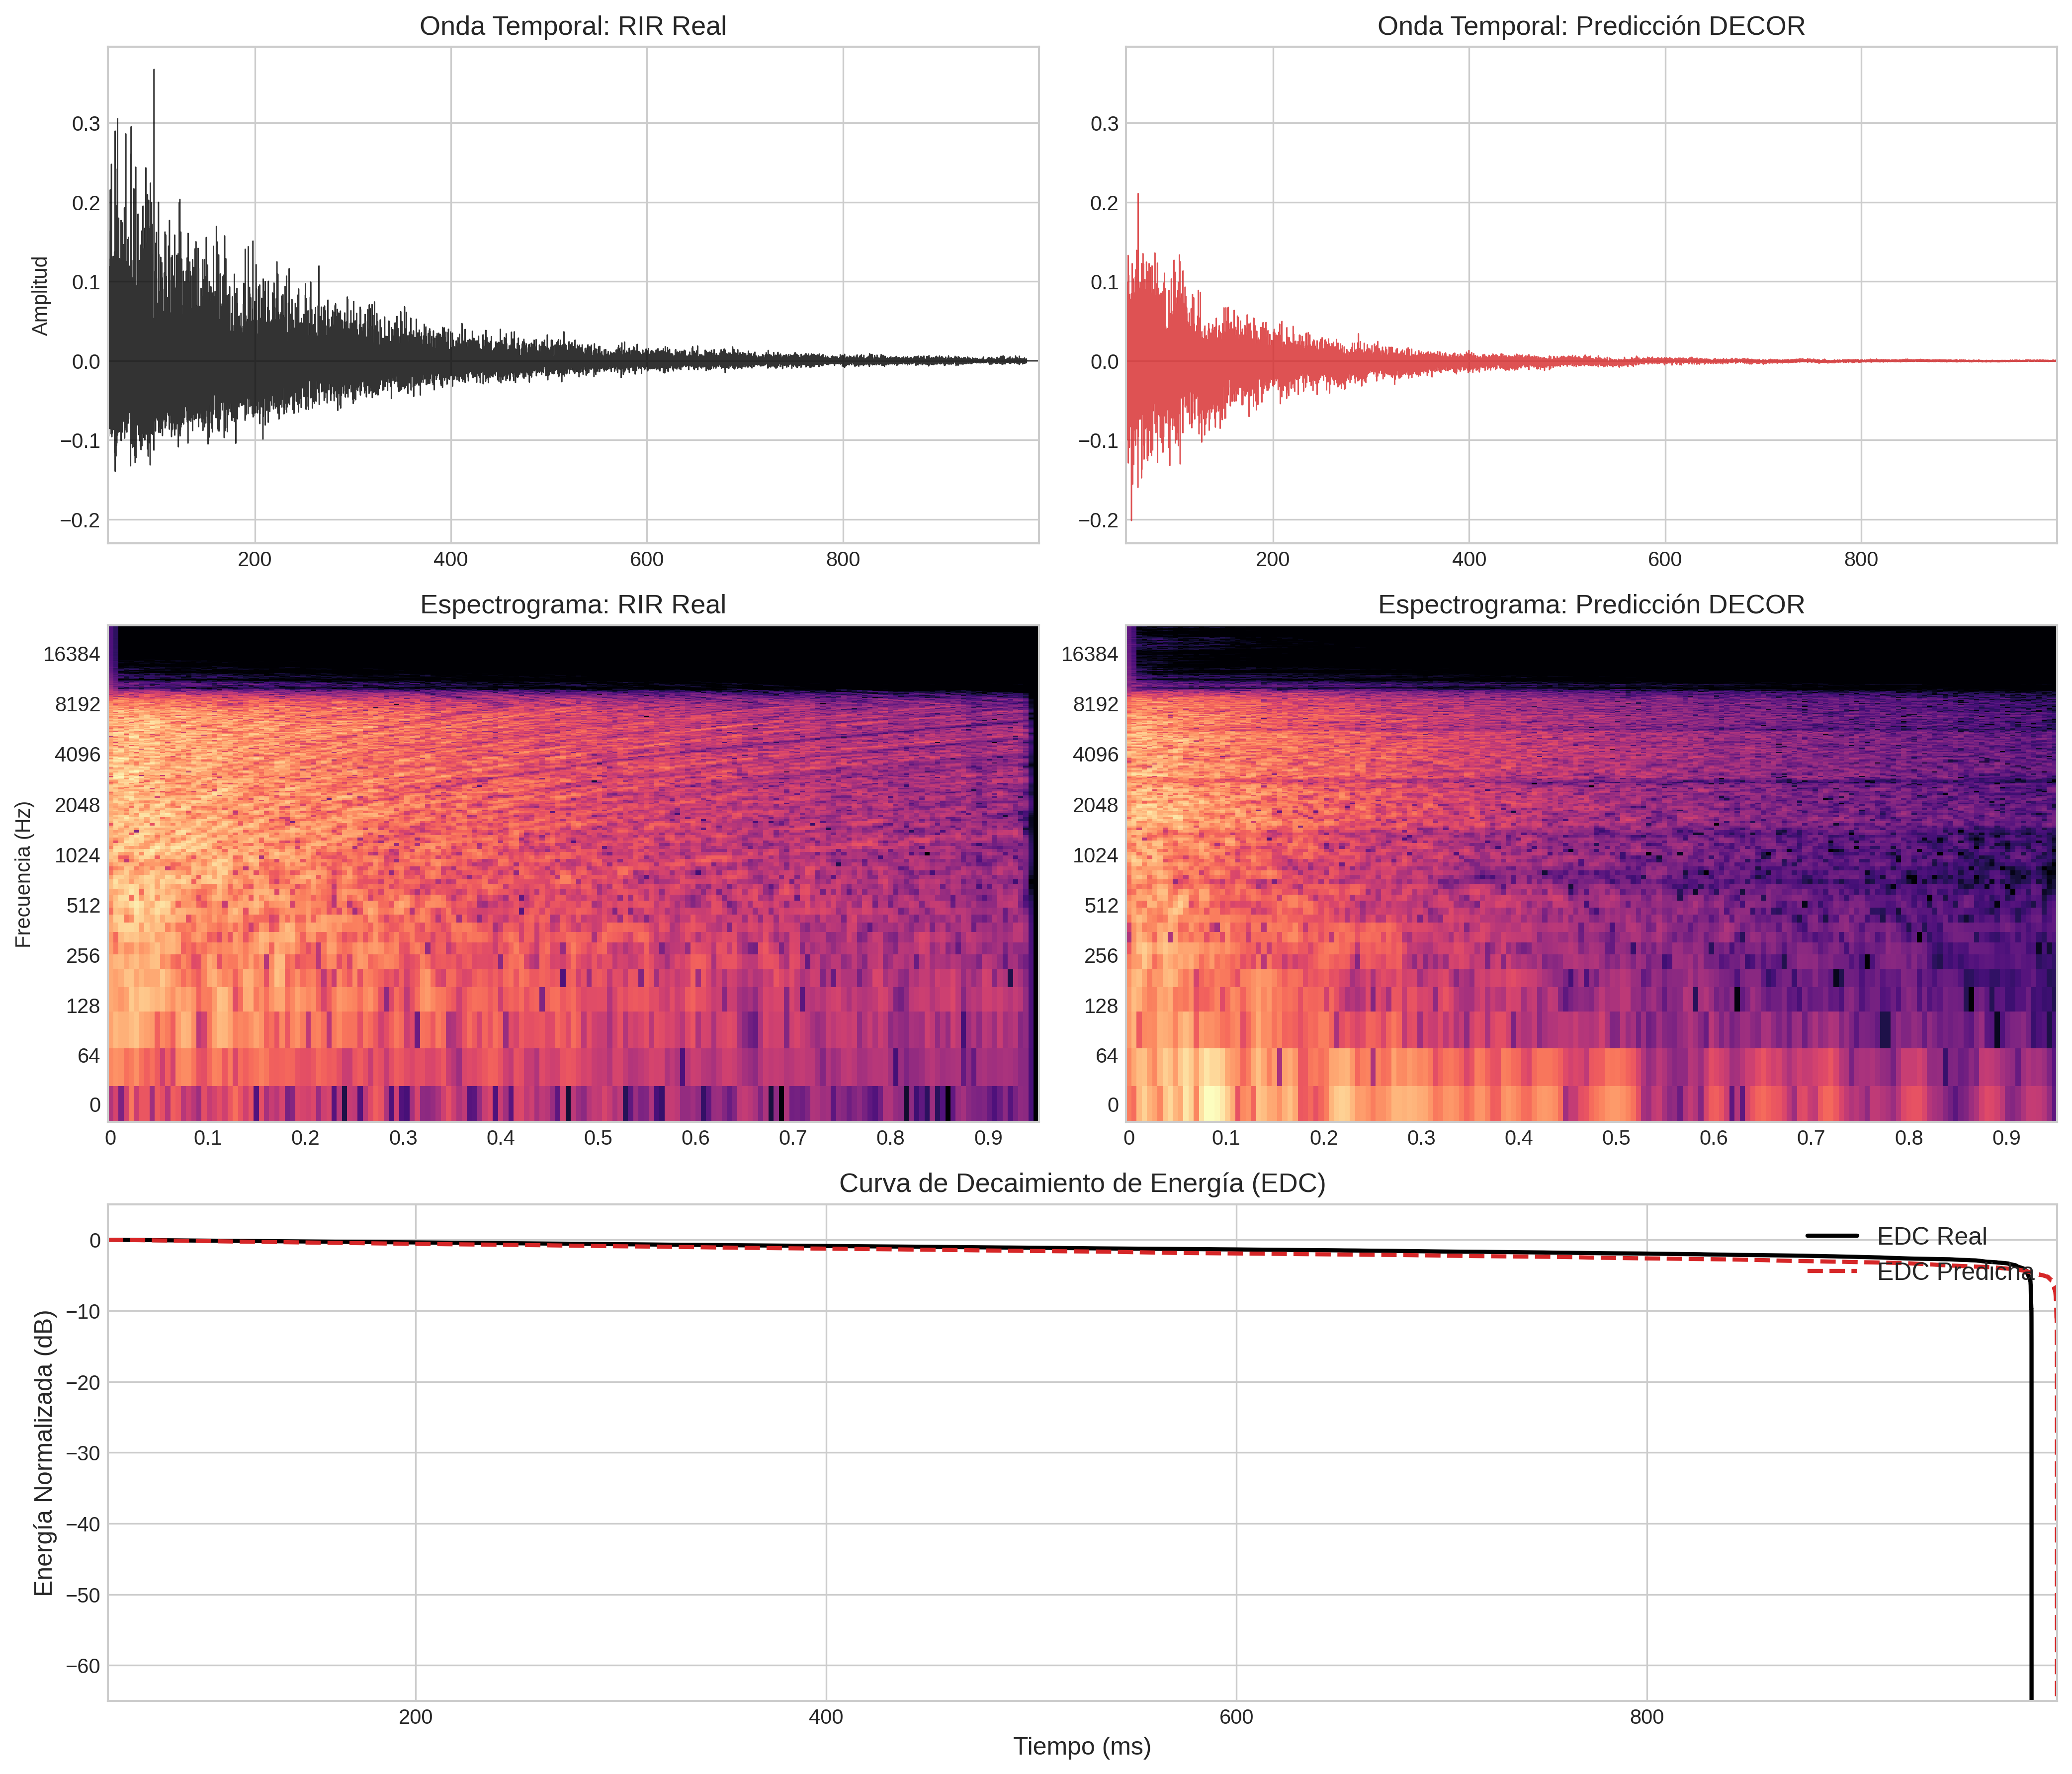
\includegraphics[width=1\textwidth]{../Figures/analisis_cualitativo.png}
\caption{Evaluación cualitativa de un caso de estudio. (Arriba) Comparativa de la forma de onda temporal. (Centro) Espectrogramas de magnitud. (Abajo) Curvas de Decaimiento de Energía (EDC).}
\label{fig:caso_estudio}
\end{figure}

Tal como se observa en la Figura~\ref{fig:caso_estudio}, la comparación de la forma de onda temporal puede sintetizarse en los siguientes puntos:

\textbf{Aciertos del modelo}
\begin{itemize}
\item \textbf{Envolvente de decaimiento.} DECOR reproduce con elevada fidelidad la estructura macro-temporal de la reverberación. La atenuación progresiva de la amplitud a lo largo del tiempo, asociada a la cola reverberante, resulta prácticamente coincidente con la respuesta real.
\item \textbf{Densidad de la cola reverberante.} A partir del régimen de campo difuso (aproximadamente desde 200 ms), la síntesis mantiene un patrón denso y estocástico coherente con la señal de referencia, convergiendo hacia niveles próximos a cero en un horizonte temporal equivalente.
\end{itemize}

\textbf{Puntos de mejora y limitaciones}
\begin{itemize}
\item \textbf{Subestimación de amplitud máxima.} La discrepancia más visible aparece en los picos iniciales: la señal real alcanza máximos superiores (del orden de 0.3), mientras que la señal estimada presenta picos más contenidos (en torno a 0.2), lo que equivale a una respuesta parcialmente atenuada en escala lineal.
\item \textbf{Pérdida de estructura fina en reflexiones tempranas.} En el intervalo inicial (aproximadamente 0--100 ms), la respuesta real presenta reflexiones tempranas discretas y bien separadas. La predicción conserva su localización global, pero las representa con mayor aglomeración y menor varianza local, reduciendo nitidez en el detalle microscópico de la onda.
\end{itemize}

En el dominio espectral, la lectura de la Figura~\ref{fig:caso_estudio} puede sintetizarse en los siguientes aspectos:

\textbf{Aciertos del modelo}
\begin{itemize}
\item \textbf{Envolvente macro y distribución de energía.} La predicción preserva la estructura global del espectrograma, reproduciendo con fidelidad tanto el impacto energético inicial como el decaimiento progresivo en el eje temporal.
\item \textbf{Decaimiento dependiente de la frecuencia.} Se mantiene un comportamiento físicamente coherente: las componentes de alta frecuencia se extinguen antes, mientras que las bandas bajas y medias conservan energía durante intervalos más prolongados.
\item \textbf{Alineación temporal del decaimiento.} El instante de agotamiento energético global se sitúa en un entorno temporal concordante con la referencia, lo que respalda una estimación consistente del tiempo reverberante efectivo.
\end{itemize}

\textbf{Puntos de mejora y limitaciones}
\begin{itemize}
\item \textbf{Efecto de suavizado.} La síntesis presenta una textura más difuminada que la señal medida, cuya microestructura estocástica resulta más rugosa en la cola tardía.
\item \textbf{Resolución modal en bajas frecuencias.} En la banda baja (aproximadamente 0--128 Hz), las trazas modales verticales se representan con menor nitidez y mayor cuantización espacial.
\item \textbf{Atenuación del fondo residual.} En el tramo final del decaimiento, la predicción tiende a suprimir con mayor intensidad el ruido de fondo tenue observado en la referencia.
\end{itemize}

La comparación de las curvas EDC, igualmente visible en la Figura~\ref{fig:caso_estudio}, puede resumirse del siguiente modo:

\textbf{Aciertos del modelo}
\begin{itemize}
\item \textbf{Seguimiento de la tendencia global.} Durante la mayor parte del eje temporal, la curva estimada se superpone de forma casi idéntica a la curva de referencia, reflejando una estimación precisa de la distribución energética macroscópica.
\item \textbf{Estabilidad sin desviaciones sistémicas.} No se observan saltos espurios, oscilaciones anómalas ni desplazamientos persistentes de nivel entre trayectorias, lo que indica normalización energética robusta.
\end{itemize}

\textbf{Puntos de mejora y limitaciones}
\begin{itemize}
\item \textbf{Divergencia en el truncamiento final.} En el entorno previo a la caída abrupta al suelo de ruido, la predicción tiende a retener energía ligeramente más tiempo o a decaer de forma menos brusca que la referencia.
\item \textbf{Sensibilidad al ruido de fondo estocástico.} La estimación del instante exacto de corte en la cola final mantiene una dificultad intrínseca elevada en modelos neuronales aplicados a audio.
\end{itemize}

En conjunto, pese a las discrepancias localizadas en la microtextura espectral y en el truncamiento final, la coincidencia global de patrones respalda que el sistema asimila con elevada precisión la dinámica energética del recinto y confirma su robustez matemática en extrapolación ciega.

